\clearpage


\section{Navigation tree and wireframe}\label{sec:navigation-tree-and-wireframe}

\subsection{Navigation tree}\label{subsec:navigation-tree}

\begin{figure}[h]
    \centering
    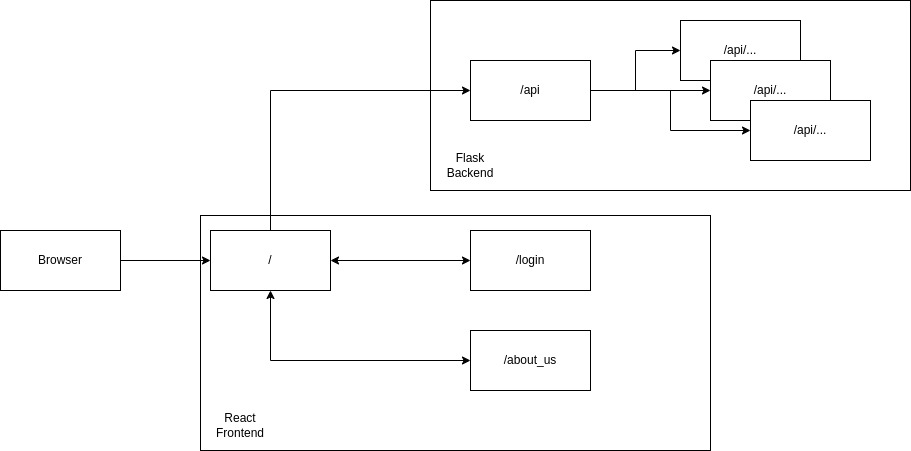
\includegraphics[width=\textwidth]{../images/navigation tree}
    \caption{Navigation tree for single-page React application with Flask backend}
    \label{fig:navigationTree}
\end{figure}
The navigation tree for this application is as shown in~\ref{fig:navigationTree}.
Deciding between a single-page application (SPA) and a multi-page application (MPA) came down to multiple concerns such as user experience and use case.
SPAs allow the user to interact with the application without having to browse through pages for actions such as log-in.
Single-page applications allow the users to view and interact with dynamic content while MPAs allow for simpler static content.

For this application, the main functionality can be displayed neatly within a single-page as shown in pre-existing applications.
As the application will also be using Websocket, the content will be dynamic and thus a single-page application approach is preferred.

There is also a separation between the front-end and back-end, with the user-interface (UI) being built in Javascript and the React library and the server being built in Python and the Flask library.
Although Flask allows to dynamically generate static HTML pages through Jinja2 Templates, there is minimal flexibility for dynamic content.
In addition, Jinja2 Templates are primarily for creating static pages which again will not be the direction for this application.
And therefore, a more suitable library such as React will be used to create the UI.

\clearpage

\subsection{Wireframe}\label{subsec:wireframe}

\begin{figure}[h]
    \centering
    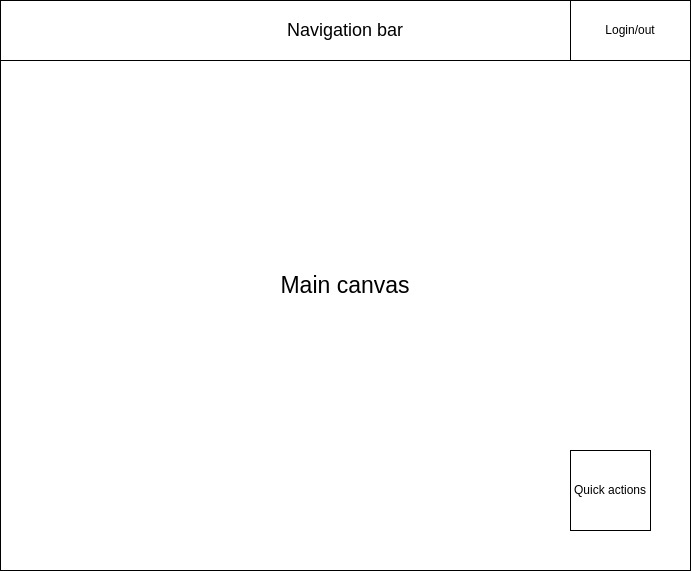
\includegraphics[width=0.8\textwidth]{../images/wireframe}
    \caption{Wireframe for application}
    \label{fig:wireframe}
\end{figure}

